\section{Track slopes: Parametric approach}
\label{sec:slopes}
%
An alternative parametric approach was also developed to model the slopes. A gaussian
fit is made to the difference between the true and reconstructed
slopes in bins of momentum. A  fit of the form
\begin{equation}
\sigma(tx) = \sqrt{A_{res}^2 + \frac{B_{ms}^2}{p^2}}
\label{eq:sloperes}
\end{equation}
 is then made to the resulting distributions of the slopes in $x$ and
 $y$ versus momentum. As example this is shown for the $y$ slopes in  Fig. \ref{fig:sloperes}. In this form the first term accounts for
the effect of detector resolution and the second for multiple
scattering. The fit, shown in Fig. \ref{fig:slopefitty},  gives $A_{res} = 7 \times 10^{-5}$ and $B_{ms} =
0.9 \mevc$. This method is simple if not perfect, in particular the quality of
the Gaussian slice fits at low $p$ is poor ($\chi^2/ndof
\sim 6$). This reflects the importance of of other variables and also
the the non-Gaussian tails in the multiple scattering distribution. 
\begin{figure}[htb!]
\begin{center}
\resizebox{3.8in}{!}{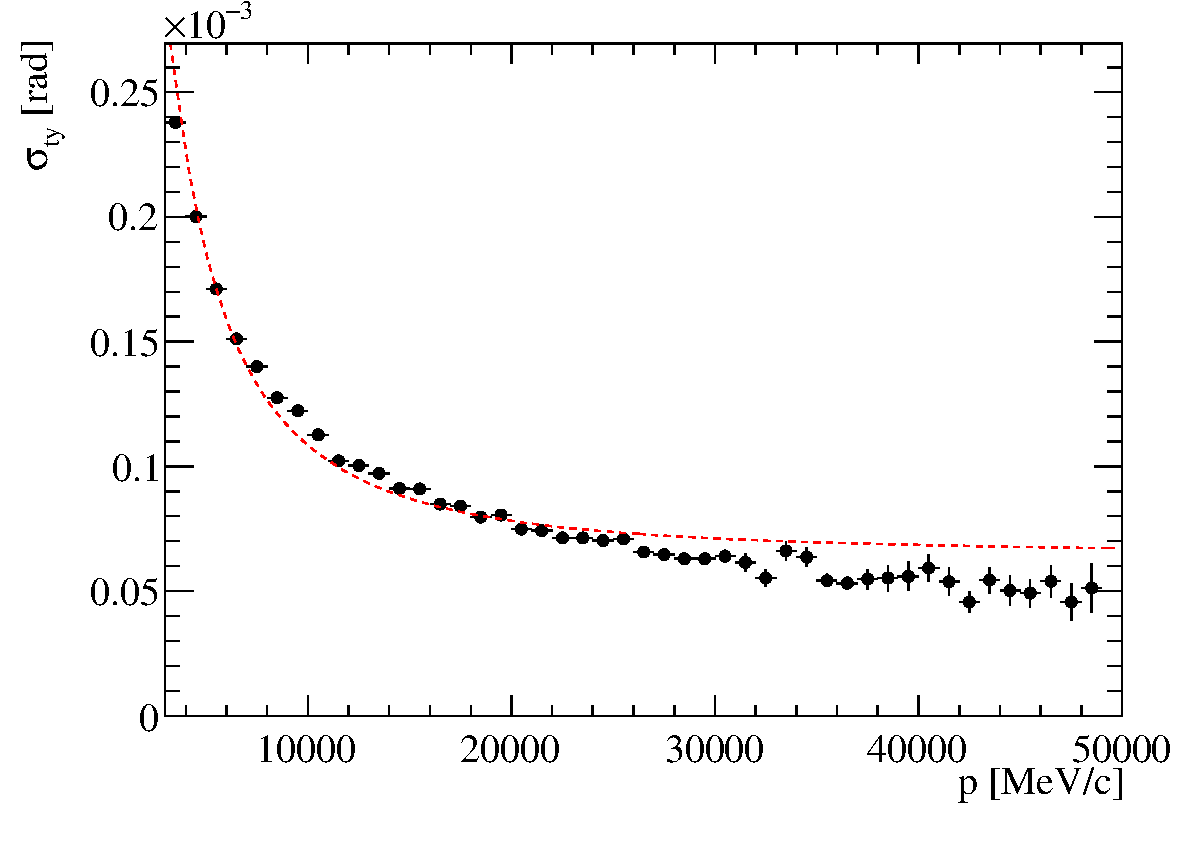
\includegraphics{figs/slopefit-ty.pdf}}
\caption{\small Track slope resolution in y versus momentum. A fit to the
  form given in Eq. \ref{eq:sloperes} is superimposed.}
\label{fig:slopefitty}
\end{center}
\end{figure}
%

As in the case of the track momentum uncertainty the pulls from this
approach are not one. The Gaussian core, which encompasses $84 \%$ of
the distribution,  has a width of 0.8  and the tail as width of 1.8.  

Other more complicated parameterizations two-dimensional binning and fitting schemes ($e.g.$ in $\pt$ and
$\eta$ bins ) were tried but found not
to improve the results significantly (whilst adding
complexity). Table~\ref{tab:valids} shows the comparision of the mass resolution
found using this approach and the full simulation for the decay modes
considered. The agreement compared to the MVA approach (Table \ref{tab:valid}) is
noticeably worse.  Hence, since this method gives worse results and is
more involved it was not considered further.

\begin{table}[htb!]
\caption{\small Comparison of the resolution found in the full
  simulation and with the emulator described in the text for several
  decay modes. }
\begin{center}
\small
\begin{tabular}{l|c|c|c|c}
Mode & Full MC Conditions & $\sigma^{fit}_m$ [$\mevcc$] &
                                                          $\sigma^{em}_m$
                                                          [$\mevcc$] &
  Ratio\\ \hline
$\chicone \rightarrow J/\psi \mu^+ \mu^-$  & 2016 & $1.66 \pm 0.01$ &
                                                                      $1.70
                                                                      \pm
                                                                      0.01$
                                                                     &
  1.02\\
$\chictwo \rightarrow J/\psi \mu^+ \mu^-$  & 2016 & $1.81 \pm 0.01$ &
                                                                      $1.87
                                                                      \pm
                                                                      0.01$
                                                                     &
  1.03\\
$\psi(2S) \rightarrow J/\psi \pi^+ \pi^-$  & 2011+12 & $2.13 \pm 0.01$
                                                        &  $2.18 \pm
                                                          0.01$ & 1.02
  \\
$X(3872) \rightarrow J/\psi \pi^+ \pi^-$  & 2016 &$2.62 \pm 0.01$ &
                                                                    $2.75
                                                                    \pm
                                                                    0.01$
                                                                     &
  1.05\\
\end{tabular}
\end{center}
\label{tab:valids}
\end{table} 
